% !TeX spellcheck = en_US

\documentclass{../UTNetLab}

\title{Bridges, LANs and the Cisco~IOS}
\labnumber{3}
\newcommand\reference{
   S. Panwar, S. Mao, J.-dong Ryoo, and Y. Li, “Bridges, LANs and the Cisco IOS,” in TCP/IP Essentials: A Lab-Based Approach, Cambridge: Cambridge University Press, 2004, pp. 61–76.
}

\begin{document}
\section*{Objectives}
\begin{itemize}
    \item The Cisco Internet Operating System (IOS) software.
    \item Configuring a Cisco router.
    \item Transparent bridge configuration and operation.
    \item The spanning tree algorithm.
\end{itemize}

\part{Exercises on Cisco~IOS}
In this lab, you need two hosts, a bridge, and two hubs, which are required to be connected as shown in \hyperref[fig:3.7]{Figure~3.7}, \hyperref[tab:3.2]{Table~3.2} and \hyperref[tab:3.3]{Table~3.3}.

\section{Network Setup}
In this exercise we build the connection to the router (see \hyperref[fig:3.7]{Figure~3.7}, \hyperref[tab:3.2]{Table~3.2} and \hyperref[tab:3.3]{Table~3.3}).

Use two hosts, two hubs, and one router (as a bridge).
Then, connect first host to the first hub and connect the first port of the bridge to the previously mentioned hub.
Now, connect the other side of the topology just like first side.

\begin{table}[H]
    \caption{Router and Host IP addresses for \hyperref[fig:3.7]{Figure~3.7} (Table~3.2\label{tab:3.2}, Table~3.3\label{tab:3.3})}
    \centering
    \begin{tabular}{ *2c|*2c|*2c }
        \hline \hline
        \multicolumn{2}{c|}{Router} & \multicolumn{2}{c|}{Host\textsubscript{A} (h0)} & \multicolumn{2}{c}{Host\textsubscript{B} (h1)}                                                \\
        eth0                        & eth1                                            & Name                                           & IP Address        & Name & IP Address        \\
        \hline
        128.238.61.1/24             & 128.238.61.2/24                                 & h0                                             & 128.238.61.100/24 & h1   & 128.238.61.101/24 \\
        % 128.238.62.2/24 & 128.238.62.3/24 & h2 & 128.238.62.102/24 & h3 & 128.238.62.103/24 \\
        % 128.238.63.3/24 & 128.238.63.4/24 & h4 & 128.238.63.104/24 & h5 & 128.238.63.105/24 \\
        % 128.238.64.4/24 & 128.238.64.5/24 & h6 & 128.238.64.106/24 & h7 & 128.238.64.107/24 \\
        \hline \hline
    \end{tabular}
\end{table}

\begin{figure}[H]
    \centering
    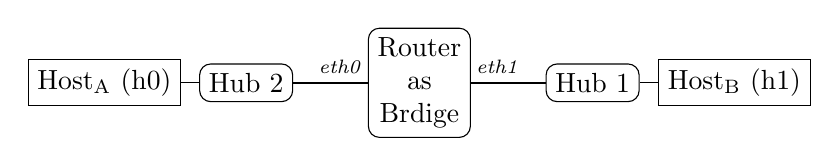
\begin{tikzpicture}
        \node[draw] (h1) at (-4,0){Host\textsubscript{A} (h0)};
        \node[draw,rounded corners] (hub2) at (-2.2,0){Hub 2};
        \node[draw,rounded corners,align=center] (router) at (0,0){Router\\as\\Brdige};
        \node[draw,rounded corners] (hub1) at (2.2,0){Hub 1};
        \node[draw] (h0) at (4,0){Host\textsubscript{B} (h1)};

        \draw (h0) -- (hub1);
        \draw (h1) -- (hub2);
        \draw[thick] (hub1) -- (router);
        \draw[thick] (hub2) -- (router);
        \draw (router) +(-1,0.2) node {\scriptsize\textit{eth0}};
        \draw (router) +(1,0.2) node {\scriptsize\textit{eth1}};
    \end{tikzpicture}
    \caption{Using a transparent bridge (Figure~3.7)}\label{fig:3.7}
\end{figure}

% ignore excersise 1 from book

\section{IOS Console}
Open Router Console (Use telnet to router from host or connect console to serial port).
In \textbf{GNS3} right click on router and open console window.
You should now be in the \textit{User EXEC} mode.

Type \lstcisco{help} to learn how to use the online help.
Study \hyperref[fig:3.6]{Figure~3.6} of reference book.
Navigate through the \textit{User EXEC}, \textit{Privileged EXEC}, \textit{Global Configuration}, and \textit{Interface Configuration} modes.
In each mode, type \lstcisco{?} to display a list of available commands and study these commands.

Type \lstcisco{show version} in the \textit{User EXEC} mode to display the Cisco~IOS banner.
Identify which Cisco~IOS Release is running in the router.
Save the Cisco~IOS banner for your lab report.

\paragraph{See} the Cisco~IOS banner.
Identify the release of the Cisco~IOS software in the router.

\part{A Simple Bridge Experiment}
\hyperref[fig:3.7]{Figure~3.7} shows a simple case of the use of bridges, which consists of two network segments connected by a bridge.
With this simple topology, we can easily capture initial BPDUs before each bridge is engaged in the spanning tree calculation.

Configure transparent bridging as in \hyperref[fig:3.7]{Figure~3.7}, \hyperref[tab:3.2]{Table~3.2} and \hyperref[tab:3.3]{Table~3.3}.
Note that the default configuration of the hosts and the bridges are different from those in the tables.
You need to change the IP addresses of the bridge interfaces,\footnote{As soon as you change the IP address of the bridge interface your host is connected to, the \lstbash{telnet} connection will be lost.
    You need to again change the IP address of all machine to be in the same subnet as the bridge interface.
    See Section~3.3.3  of reference book.} as well as set the bridge group and enable the spanning tree algorithm (see the previous section on bridge configuration).
Do the following experiments.

Config Cisco Router as transparent Bridge:
\begin{lstlisting}[language={cisco}]
config term
    no ip routing
    bridge 1 protocol ieee ! for STP protocol
    int f0/0
        ip addr 128.238.61.1 255.255.255.0
        bridge-group 1
        no shut
        exit
    int f0/1
        ip addr 128.238.61.2 255.255.255.0
        bridge-group 1
        no shut
        end
Ctrl+Z
    \end{lstlisting}

\section{Bridge Packet}
Run \lstbash{tcpdump -en ip proto 1} on the \textit{h0} and the \textit{h1} machine.
Send \lstbash{ping} messages to \textit{h1} machine from the \textit{h0}: \lstbash[emph={h1,netlab}]{ping -sv h1.netlab}.
After receiving the tenth echo reply, quit the \lstbash{ping} process, and save the \lstbash{tcpdump} outputs from both machines.

During this exercise, don’t run \lstbash{ping} programs at the same time from other host.
For clean results, do your experiments in turn.

\begin{report}
    \item What are the IP and MAC addresses of a packet that went from the \textit{h0} machine to the bridge?
    What are the IP and MAC addresses of a packet that went from the router to the \textit{h1} machine?

    \item Answer the same questions, but for the echo reply that was returned from the \textit{h1} machine.

    \item Using the \lstbash{tcpdump} outputs from both machines, calculate the average delay that a packet experienced in the bridge.
    \footnote{Note that the system times of the two machines might be different.}
\end{report}

Show all the steps and submit the \lstbash{tcpdump} outputs with your report.

\section{STP/BPDU Packet}
Run \lstbash{tcpdump -e -c 5 ether multicast -vv} on all machines to capture 2 BPDUs messages generated by the bridge.
Save the BPDUs for the lab report.

%    You need to collect all the different BPDUs from all group in your lab.
%    At this time, save your BPDU capture output.

%    In our next step,  you get BPDUs from other gropu.
% explain stp and bpdu

You should collect BPDUs in this exercise.
These BPDUs will be helpful when studying the spanning tree algorithm later in this chapter.

\begin{report}
    \item How frequently (in seconds) does a bridge sends its BPDUs?

    \item Submit the two different BPDUs you saved.
    Identify the values of root ID, root path cost, bridge ID, and port ID for each BPDU\footnote{You may check the physical addresses of network interfaces.
        You need the MAC addresses to help analyze the BPDUs.} (may need to check BPDU message format \hyperref[fig:3.4]{Figure~3.4}).
\end{report}

\begin{figure}[H]
    \centering
    \resizebox{0.9\textwidth}{!}{
        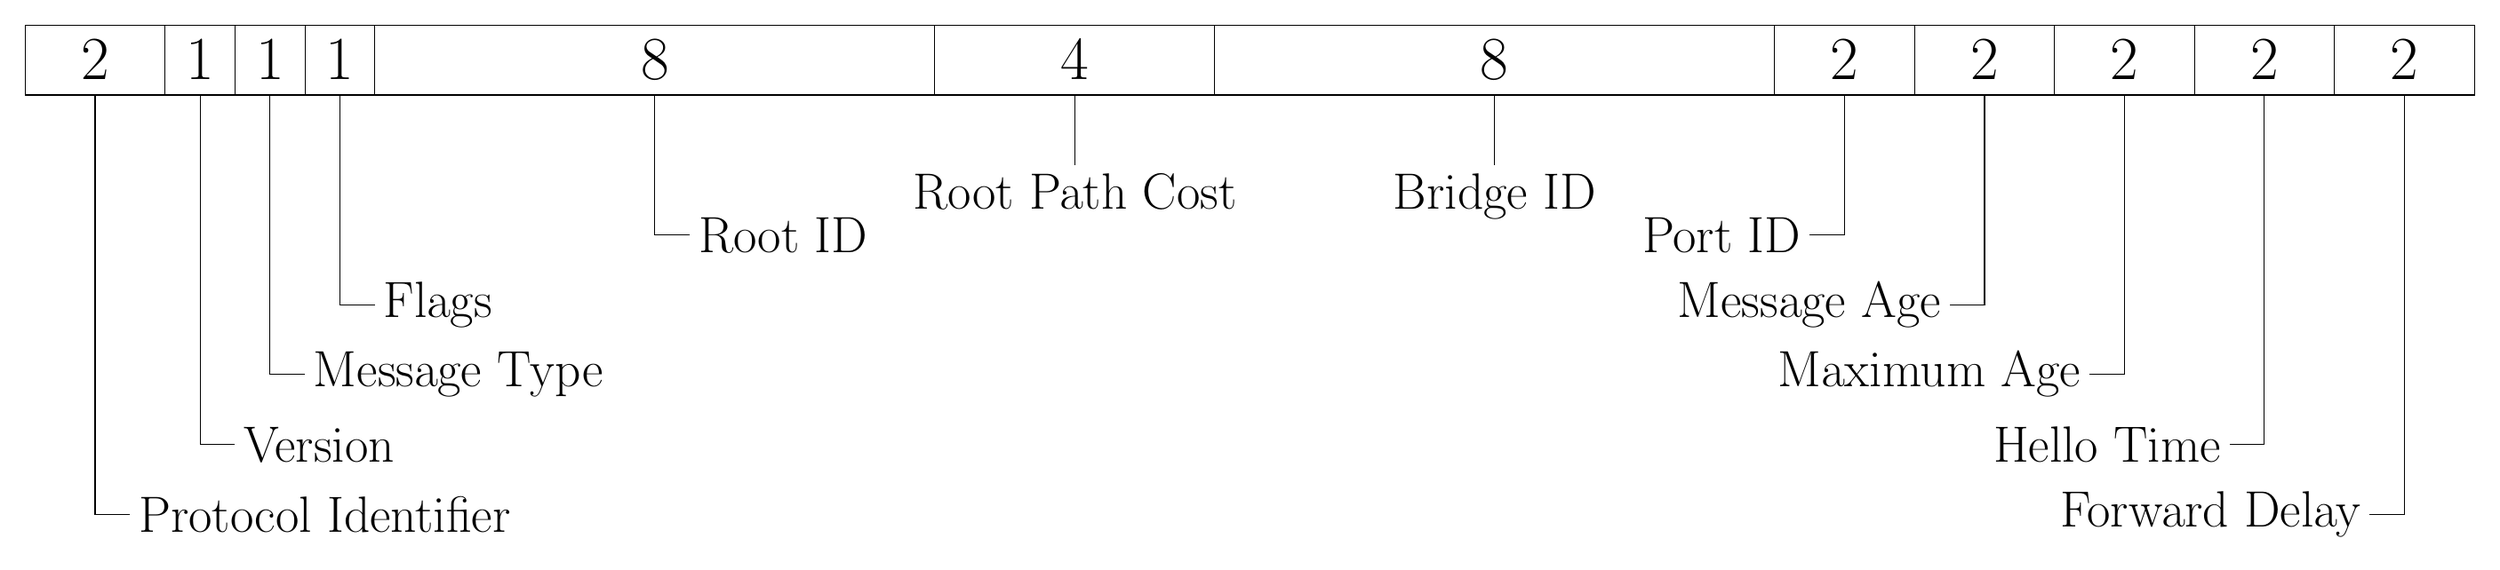
\begin{tikzpicture}
            \draw (0,0)
            rectangle ++(2,1) node[pos=0.5] {\Huge 2} ++(-0.5*2,-1) |- +(0.5,-1*6) node[anchor=west] {\huge Protocol Identifier} ++(0.5*2,0)
            rectangle ++(1,1) node[pos=0.5] {\Huge 1} ++(-0.5*1,-1) |- +(0.5,-1*5) node[anchor=west] {\huge Version} ++(0.5*1,0)
            rectangle ++(1,1) node[pos=0.5] {\Huge 1} ++(-0.5*1,-1) |- +(0.5,-1*4) node[anchor=west] {\huge Message Type} ++(0.5*1,0)
            rectangle ++(1,1) node[pos=0.5] {\Huge 1} ++(-0.5*1,-1) |- +(0.5,-1*3) node[anchor=west] {\huge Flags} ++(0.5*1,0)
            rectangle ++(8,1) node[pos=0.5] {\Huge 8} ++(-0.5*8,-1) |- +(0.5,-1*2) node[anchor=west] {\huge Root ID} ++(0.5*8,0)
            rectangle ++(4,1) node[pos=0.5] {\Huge 4} ++(-0.5*4,-1) |- +(0,-1*1)   node[anchor=north] {\huge Root Path Cost} ++(0.5*4,0)
            rectangle ++(8,1) node[pos=0.5] {\Huge 8} ++(-0.5*8,-1) |- +(-0,-1*1)  node[anchor=north] {\huge Bridge ID} ++(0.5*8,0)
            rectangle ++(2,1) node[pos=0.5] {\Huge 2} ++(-0.5*2,-1) |- +(-0.5,-1*2) node[anchor=east] {\huge Port ID} ++(0.5*2,0)
            rectangle ++(2,1) node[pos=0.5] {\Huge 2} ++(-0.5*2,-1) |- +(-0.5,-1*3) node[anchor=east] {\huge Message Age} ++(0.5*2,0)
            rectangle ++(2,1) node[pos=0.5] {\Huge 2} ++(-0.5*2,-1) |- +(-0.5,-1*4) node[anchor=east] {\huge Maximum Age} ++(0.5*2,0)
            rectangle ++(2,1) node[pos=0.5] {\Huge 2} ++(-0.5*2,-1) |- +(-0.5,-1*5) node[anchor=east] {\huge Hello Time} ++(0.5*2,0)
            rectangle ++(2,1) node[pos=0.5] {\Huge 2} ++(-0.5*2,-1) |- +(-0.5,-1*6) node[anchor=east] {\huge Forward Delay} ++(0.5*2,0)
            ;
        \end{tikzpicture}
    }
    \caption{BPDU message format (Figure~3.4)}\label{fig:3.4}
    {\footnotesize The numbers indicate the field length in byte.}
\end{figure}

\part{Spanning Tree Exercises}
\label{sec:spanning-tree}
In this section, we will use \hyperref[fig:3.8]{Figure~3.8} as our network topology.
You need to change the IP addresses of the bridge interfaces, as well as that of all machines.
Refer to Section~3.3.4 of reference book on how to configure a transparent bridge.
Also see Section~3.3.3 of reference book on how to handle a frozen telnet session after you change the bridge IP address.

Upon being started, a transparent bridge learns the network topology by analyzing source addresses of incoming frames from all attached networks.
The next exercise shows the process by which a transparent bridge builds its filtering database.

You can read \autoref{appendix:spanningTree} and \autoref{appendix:bpdu} to learn how Spanning Tree Algorithm work.
\begin{figure}[H]
    \centering
    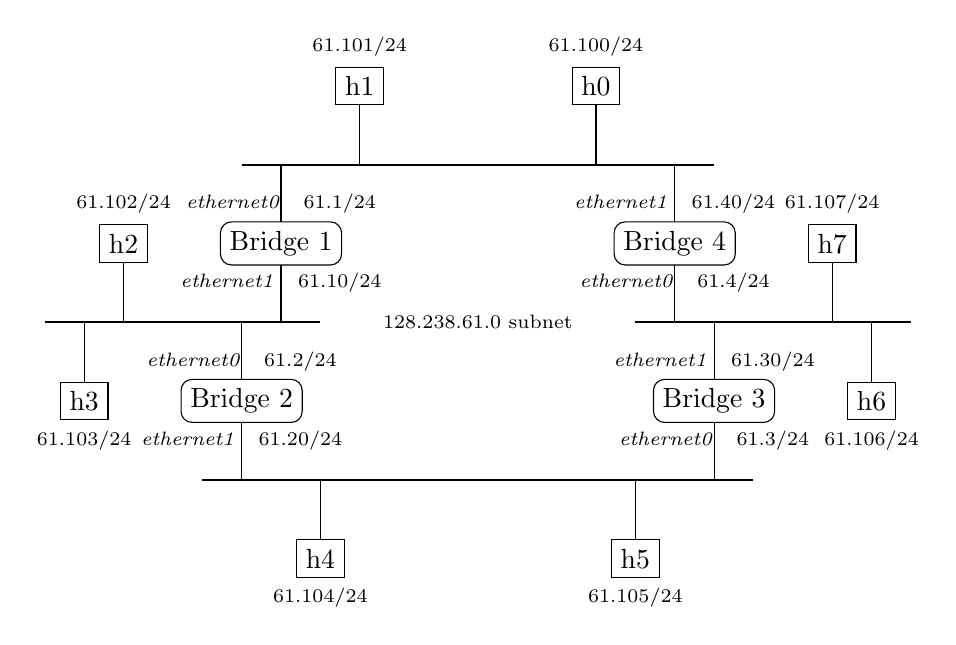
\begin{tikzpicture}
        \node at (0,0) {\scriptsize 128.238.61.0 subnet};
        \draw (2.5,1) node[draw,fill=white,rounded corners] (br4) {Bridge 4}
        -- +(0,-1)
        -- +(0,+1)
        +(0,0.5) node {\scriptsize\textit{ethernet1}\quad 61.40/24}
        +(0,-0.5) node {\scriptsize\textit{ethernet0}\quad 61.4/24}
        ;
        \draw (3,-1) node[draw,fill=white,rounded corners] (br3) {Bridge 3}
        -- +(0,-1)
        -- +(0,+1)
        +(0,0.5) node {\scriptsize\textit{ethernet1}\quad 61.30/24}
        +(0,-0.5) node {\scriptsize\textit{ethernet0}\quad 61.3/24}
        ;
        \draw (-2.5,1) node[draw,fill=white,rounded corners] (br1) {Bridge 1}
        -- +(0,-1)
        -- +(0,+1)
        +(0,-0.5) node {\scriptsize\textit{ethernet1}\quad 61.10/24}
        +(0,0.5) node {\scriptsize\textit{ethernet0}\quad 61.1/24}
        ;
        \draw (-3,-1) node[draw,fill=white,rounded corners] (br2) {Bridge 2}
        -- +(0,-1)
        -- +(0,+1)
        +(0,-0.5) node {\scriptsize\textit{ethernet1}\quad 61.20/24}
        +(0,0.5) node {\scriptsize\textit{ethernet0}\quad 61.2/24}
        ;
        \draw (4.5,1) node[draw,fill=white] {h7}
        -- +(0,-1)
        +(0,0.5) node {\scriptsize 61.107/24}
        ;
        \draw (5,-1) node[draw,fill=white] {h6}
        -- +(0,1)
        +(0,-0.5) node {\scriptsize 61.106/24}
        ;
        \draw (-4.5,1) node[draw,fill=white] {h2}
        -- +(0,-1)
        +(0,0.5) node {\scriptsize 61.102/24}
        ;
        \draw (-5,-1) node[draw,fill=white] {h3}
        -- +(0,1)
        +(0,-0.5) node {\scriptsize 61.103/24}
        ;
        \draw (-1.5,3) node[draw,fill=white] {h1}
        -- +(0,-1)
        +(0,0.5) node {\scriptsize 61.101/24}
        ;
        \draw (1.5,3) node[draw,fill=white] {h0}
        -- +(0,-1)
        +(0,0.5) node {\scriptsize 61.100/24}
        ;
        \draw (-2,-3) node[draw,fill=white] {h4}
        -- +(0,1)
        +(0,-0.5) node {\scriptsize 61.104/24}
        ;
        \draw (2,-3) node[draw,fill=white] {h5}
        -- +(0,1)
        +(0,-0.5) node {\scriptsize 61.105/24}
        ;
        \draw[thick] (2,0) -- +(3.5,0);
        \draw[thick] (-2,0) -- +(-3.5,0);
        \draw[thick] (-3,2) -- +(6,0);
        \draw[thick] (-3.5,-2) -- +(7,0);
    \end{tikzpicture}
    \caption{Bridge experiment network (Figure~3.8)}\label{fig:3.8}
\end{figure}

\section{Multi Bridge Path}
After configuring the network in \hyperref[fig:3.8]{Figure~3.8}, open the \textit{bridge 1} console.

Get to the \textit{Privileged EXEC}\footnote{use \lstcisco{enable} command to active \textit{Privileged EXEC}} mode (is activated by default in \textbf{GNS3}).
Type \lstcisco{show bridge} to see the entries in the bridge forwarding database.

Whenever you \lstbash{ping} or \lstbash{telnet} from the \textit{h0} to a host that is not in the table (table form bridge 1), observe how the filtering database in the bridge is expanded.

You may use the \lstcisco[emph={group}]{clear bridge group} command to remove any learned entries from the filtering database, if you see a full filtering database or if you want to repeat the above exercise.

\begin{report}
    \item From the output of \lstcisco{show bridge}, identify which bridge ports are blocked, and which ports are in the forwarding state for each bridge.
\end{report}

\section{STP Process}
Using \lstbash{tcpdump -ex ether multicast -vv} on all LAN segments, capture the BPDU packet flowing on your network segment.

To collect all BPDU packets from start time, you need restart (reload) all router.

Open console of each bridge to collect the \lstcisco{show bridge} outputs.

\begin{report}
    \item Submit the four different BPDUs (from four network sections) you saved.
    Identify the values of root ID, root path cost, bridge ID, and port ID for each BPDU.

    \item Based upon the initial BPDUs saved in \nameref{sec:spanning-tree}, draw the spanning tree seen by the BPDUs (or explain root node and its child).
    Identify the root ports and the root path cost (in hop counts) for each bridge.
    %           Identify the state of each bridge port (blocking or forwarding).
    Based on Spanning tree algorithm section in the reference book (section 3.2.3 page 63), explain how root node selected?

    \item Write the final BPDUs you collected using the three-tuple format: \textit{{root ID, root path cost, bridge ID}}.

    \item Once you have the spanning tree, justify it using the four final BPDUs collected in this exercise and/or the output of the \lstcisco{show bridge} command.
\end{report}


\section{STP over Topology Dynamics}
First, send \lstbash{ping} messages from the \textit{h3} to \textit{h4}, while \lstbash{tcpdump} is running.
Let the two programs run during this exercise.

Then, shutdown (disconnect) the cable from the \textit{ethernet0} (equal to \textit{FastEthernet0/0} or \textit{f0/0}) port of \textit{Bridge2} from the hub (by \lstcisco{shut} in the router interface configuration mode), and get system time (\lstbash{date}, \lstbash{date '+\%D \%T.\%N'} or \lstbash{date +\%s\%N} to get nano seconds) on the \textit{h3} or the \textit{h4} to get the current time.

Observe the \lstbash{ping} and \lstbash{tcpdump} windows.
When the connection is reestablished, get the \lstbash{time} again.
How long does it take the spanning tree algorithm to react to the change in the topology?

Once you can successfully reach other hosts, get to the bridges to run \lstcisco{show bridge} to collect the port states.
Also collect BPDUs from all the LAN segments as you did in the previous exercise.

After every student has collected the required data, connect the cable to the original position.
Again, measure the time it takes for the bridges to adapt to the new change.

\begin{report}
    \item Draw the new tree formed after the cable was disconnected, based on the BPDUs you collected in this exercise.
    Specify the state of each bridge port.
\end{report}

\part{Exercise on the Cisco~IOS Web Browser UI}
\section{Cisco~IOS HTTP REST API}
In this section we create simple network with a router and one gui host with \textit{Internet Browser}.

\begin{figure}[H]
    \centering
    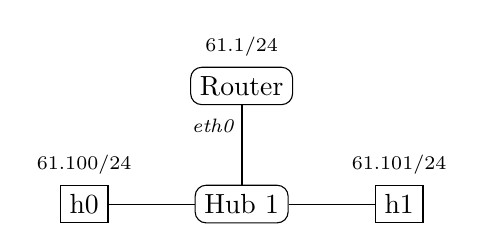
\begin{tikzpicture}
        \node[draw,rounded corners,align=center] (router) at (0,1.5){Router};
        \node[draw,rounded corners] (hub1) at (0,0){Hub 1};
        \node[draw] (h1) at (2,0){h1};
        \node[draw] (h0) at (-2,0){h0};

        \draw (h0) -- (hub1);
        \draw (h1) -- (hub1);
        \draw[thick] (hub1) -- (router);
        \draw (router) +(-0.35,-0.5) node {\scriptsize\textit{eth0}};
        \draw (router) +(0,0.5) node {\scriptsize 61.1/24};
        \draw (h1) +(0,0.5) node {\scriptsize 61.101/24};
        \draw (h0) +(0,0.5) node {\scriptsize 61.100/24};
    \end{tikzpicture}
    \caption{Two gui host with router (Figure two GUI)}
    \label{fig:two-gui}
\end{figure}

You can also configure a router using the web browser UI.
To enable the web server, open the router console and config as below  in the \textit{Global Configuration} mode.

\begin{lstlisting}[language={cisco},emph={netlab}]
R1# config term
R1(config)# aaa new-model
R1(config)# aaa authentication login default local
R1(config)# aaa authorization exec default local
R1(config)# username netlab privilege 15 password netlab
R1(config)# ip http server
R1(config)# ip http secure-server
R1(config)# ip http authentication local
    \end{lstlisting}

Next, start a web browser (e.g. \textit{Mozilla FireFox} in Linux) in your host, and enter the IP address of the router interface (\url{http://128.238.61.1}).
When prompted, enter \texttt{netlab} for user name and password.
Then you can browse the router configuration web pages and configure the router there.


\newpage
\appendix

\section{Spanning Tree Algorithm}
\label{appendix:spanningTree}
The spanning tree algorithm defined in the IEEE 802.1d standard is used in bridged networks to build trees dynamically.
It works as follows.

\begin{enumerate}
    \item Each bridge is assigned a unique identifier, and each port of a bridge is assigned an identifier unique to that bridge. Typically, the identifier of a bridge is a priority concatenated with one of the bridge ports’ MAC
          address, and the identifier of a port is a priority concatenated with a port index local to the bridge.
          Each bridge port has a corresponding path cost, which indicates the cost to transfer a frame to an attached network segment through that port.

    \item Select the root bridge, which is the one with the lowest-value bridge identifier.
          The ID of the root is called the root ID.

    \item Each bridge selects its root port.
          The root port of a bridge is the port from which the root bridge can be reached with the least aggregate path cost (called the root path cost).

    \item Determine the designated bridges and the designated ports.
          Each network segment is associated with a designated bridge, which provides the shortest path to the root bridge and is the only bridge allowed to forward frames to and from the root.
          The port connecting a designated bridge to the network segment is a designated port.
          If more than one bridge provides the same root path cost, the bridge with the lowest-valued bridge identifier is selected as the designated bridge.

    \item Only the root ports and designated ports of the bridges are allowed to forward frames.
          All other bridge ports are blocked.

    \item The above steps are repeated whenever the network topology changes.
\end{enumerate}

\section{Bridge Protocol Data Units}
\label{appendix:bpdu}
To implement the spanning tree algorithm in a distributed manner, bridges exchange configuration information using a message called bridge
protocol data units (BPDUs).
The format of a BPDU message is given in Fig~3.4 with the definition of the fields given below.

\begin{itemize}
    \item \textit{Protocol Identifier}, \textit{Version}, and \textit{Message Type}:
          These three fields are always set to 0.

    \item \textit{Flags}: The least significant bit, called the Topology Change (TC) bit, is set to signal a topology change.
          The most significant bit is to acknowledge receipt of a BPDU with the TC bit set.
          The remaining six bits are not used.

    \item \textit{Root ID}: Identifies the root bridge by listing its 2-byte priority followed by a 6-byte Ethernet address.
          The priority value can be set in the Global Configuration mode.
          The default priority is 0x8000.

    \item \textit{Root Path Cost}: The path cost to the root bridge.

    \item \textit{Bridge ID}: The identifier of the bridge sending the message.
          Port ID: Each bridge port has a unique 2-byte identifier.
          The first byte is the priority, which is configurable, while the second byte is a number assigned to the port.

    \item \textit{Message Age}:1 Specifies the amount of time since the root originally sent the BPDU on which the current configuration message is based.

    \item \textit{Maximum Age}:1 Indicates when the spanning tree topology is recalculated if a bridge does not hear BPDUs from the root bridge.
          The default value is 15 seconds.

    \item \textit{Hello Time}:1 Provides the time period between two BPDUs from the root bridge.
          The default value is 1 second.

    \item \textit{Forward Delay}:1 provides the amount of time that bridges should wait before switching a port from the blocking state to forwarding state.
          If a bridge port switches state too soon, not all network links may be ready to change their state, and loops can occur.
          The default value is 30 seconds.
\end{itemize}

\end{document}